%!TEX program = xelatex
%!BIB program = bibtex
\documentclass[cn,black,12pt,normal]{elegantnote}
\usepackage{float}
\usepackage{hyperref}
\usepackage{amsmath}
\usepackage{amsfonts}
\usepackage{amssymb}
\usepackage{siunitx}[=v2]
\usepackage{fancyhdr}
\usepackage{newtxtext}
\usepackage{algorithm}
\usepackage{algorithmic}
\newcommand{\uct}[1]{\textsuperscript{\textsuperscript{\cite{#1}}}}
\renewcommand{\tablename}{\textbf{Table}}
\renewcommand{\figurename}{Figure.}
\renewcommand{\refname}{References}
\renewcommand{\contentsname}{Contents}
\renewcommand{\versiontext}{Version: }
\renewcommand{\updatetext}{Update: }
\PassOptionsToPackage{no-math}{fontspec}
\lstset{basicstyle=\footnotesize\ttfamily\color[RGB]{50,0,130},numbers=none,frame=trBL}

\sisetup{mode=text}
\sisetup{range-phrase = \text{ \textasciitilde }}
\pagestyle{fancy}
\fancyhead[L]{School of Software Engineering, Tongji University}
\fancyhead[R]{Data Structure Projects}
\renewcommand{\headrulewidth}{1pt}

\title{Famliy Tree\\家谱管理系统}
\author{1951510\; 姜文渊}
\institute{\small \url{https://github.com/jwyjohn/Jwy_DataStructureHomework}}
\version{0.50}
\date{\today}

\begin{document}

\maketitle

\textbf{Data structure involved:} Tree

\textbf{Algorithms involved:} Recursive procedure

\tableofcontents

\newpage

\section{Introduction}
A family tree, also called a genealogy or a pedigree chart, is a chart representing family relationships in a conventional tree structure. More detailed family trees, as used in medicine and social work, are known as genograms.\uct{wiki:Family_tree}

A tree is a widely used abstract data structure that simulates a hierarchical structure (compared with linear data structures like arrays, linked lists, stacks and queues), with a root value and subtrees of children with a parent node, represented as a set of linked nodes. A tree data structure can be defined \textbf{recursively} as a collection of nodes, where each node is a data structure consisting of a value and a list of references to nodes. The start of the tree is the "root node" and the reference nodes are the "children".\uct{wiki:Tree_(data_structure)}

Since a family tree is a typical \textbf{hierarchical structure}, using trees to store and manage it can be of convenience on a computer system. In this project, the author built a demo for manipulating a family tree, with operations like add a member, remove a member, rename a member and display the full family tree.

\section{Demostration}

\subsection{Compile and run the program}

On linux platform with \lstinline{make} and a \lstinline{g++} which supports C++ 11 Standard, just \lstinline{cd} to the \lstinline{./linux} and run \lstinline{make build}. The binary executable will be generated in the same directory named as \lstinline{a.out} or \lstinline{mysort}, according to the configurations in the \lstinline{Makefile}. Use \lstinline{./a.out} or or \lstinline{./mysort} to run the program.

\textbf{CAUTION} On windows platforms, the initializetion of a pointer may cause some problems depending on your platform, so it is recommended to compile and run the code on Linux systems.

The program is an interactive shell, where you can input commands and get results.

\begin{figure}[H]
    \centering
    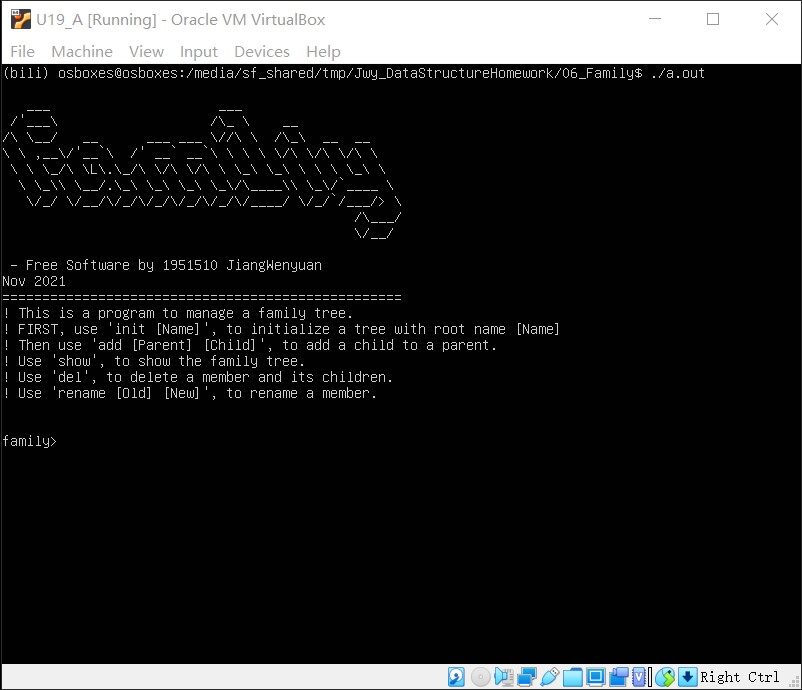
\includegraphics[width=0.7\linewidth]{image/f01.jpg}
    \caption{The user interface of the program}
\end{figure}

Usage of commands can be found on the main screen, and the \lstinline{help} command can give you information about theses commands.  All available commands is listed below.

\begin{enumerate}
    \item \lstinline{help} : Show help for a certain command.
    \item \lstinline{exit} : Exit the program.
    \item \lstinline{init [name]} : Set the name of the root of the family tree.
    \item \lstinline{add [child] [parent]} : Add a child to a node of the family tree.
    \item \lstinline{del [name]} : Delete a person (together with its children) from the family tree.
    \item \lstinline{rename [name] [newname]} : Rename a node in the family tree.
    \item \lstinline{show} : Display the family tree.
\end{enumerate}
Note that if a user inputs invalid commands or arguments, the program will be robust enough (at least to some extent) to detect the exception and return an error message. Detailed Demostration of this feature can be explored when using this program.

\subsection{initializetion and adding members to the family tree}

Type \lstinline{init Jocab} to initialize a family tree with the root named Jacob. Then use \lstinline{add [child] [parent]} to add some members.

\begin{figure}[H]
    \centering
    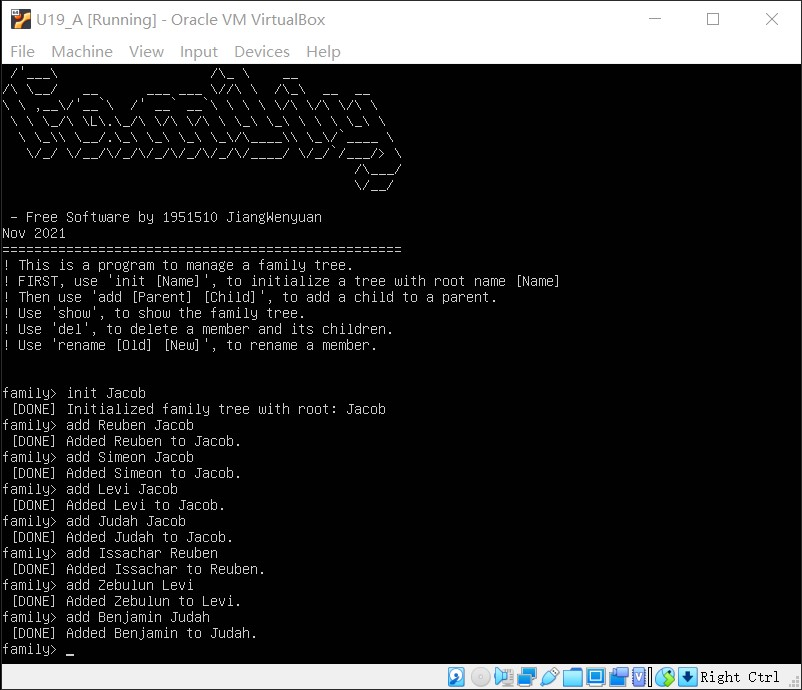
\includegraphics[width=0.7\linewidth]{image/f02.jpg}
    \caption{Adding members to the tree}
\end{figure}

To examine our family tree, use \lstinline{show}.

\begin{figure}[H]
    \centering
    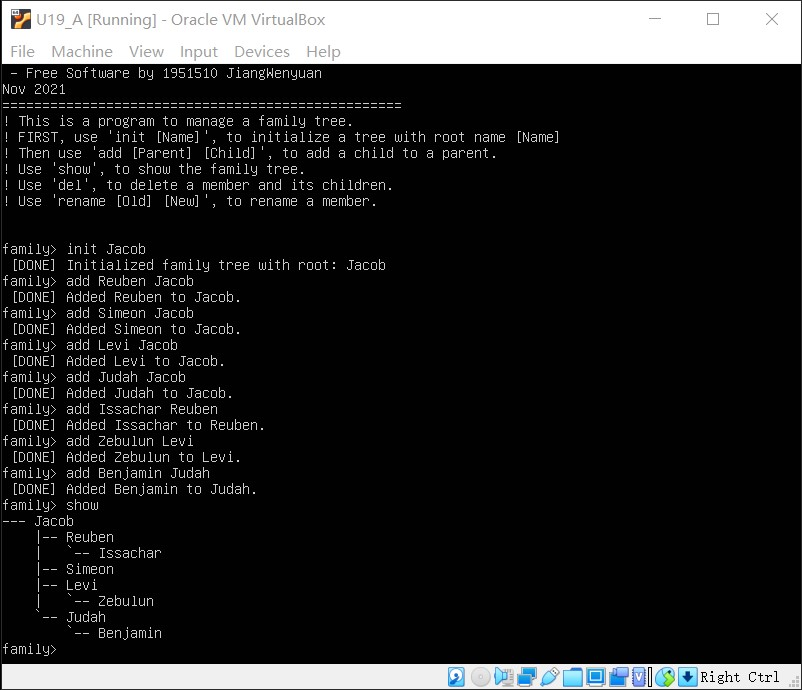
\includegraphics[width=0.7\linewidth]{image/f03.jpg}
    \caption{Use \lstinline{show} to view our family tree}
\end{figure}

\subsection{Removal and renaming}

After adding Dan to the family tree, type \lstinline{del Dan} to remove him, and the result can be seen using \lstinline{show}.
\begin{figure}[H]
    \centering
    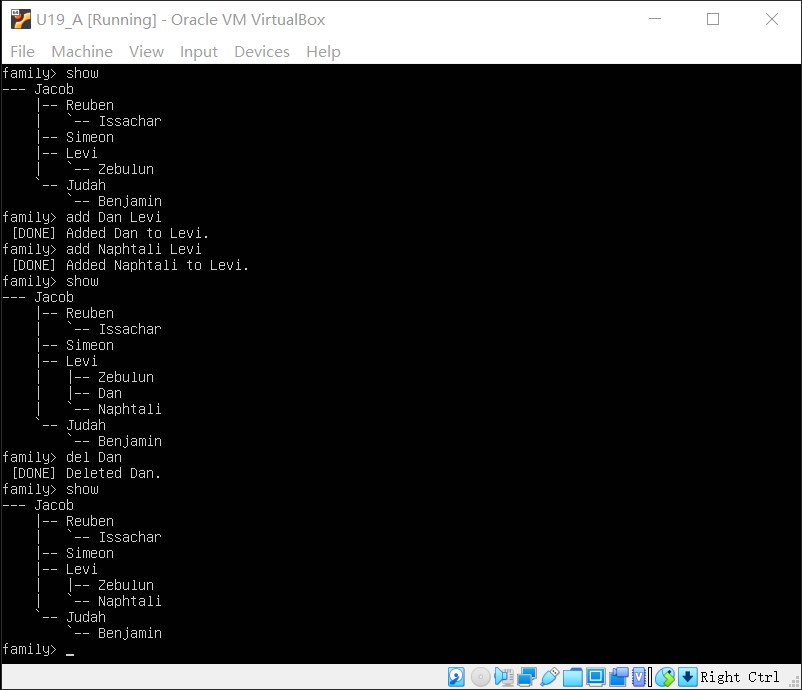
\includegraphics[width=0.7\linewidth]{image/f04.jpg}
    \caption{Use\lstinline{del Dan} to remove a member}
\end{figure}
\begin{figure}[H]
    \centering
    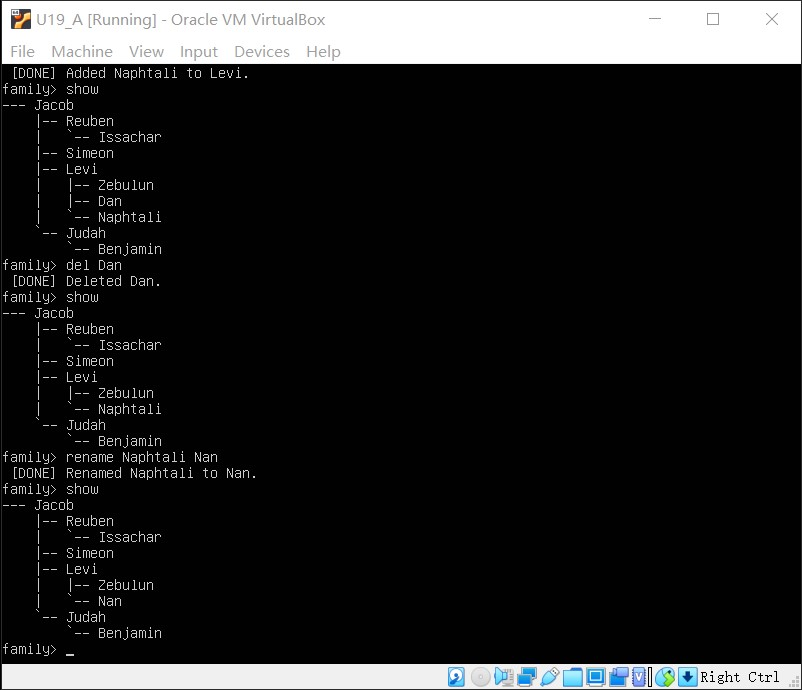
\includegraphics[width=0.7\linewidth]{image/f05.jpg}
    \caption{Renaming a member}
\end{figure}
Use \lstinline{rename Naphtali Nan} to rename a member named Naphtali to Nan, and the result can be seen using \lstinline{show}.


\section{About trees}

Many applications of trees (including this one) have more or less taken advantage on their hierarchical nature, and the examples are:
\begin{enumerate}
    \item File systems used to store data on hard drives. (B-Trees)
    \item Abstract syntax trees for computer languages.
    \item Parse trees for human languages.
    \item Document Object Models of XML and HTML documents, or JSON and YAML documents.
    \item Binary search trees.
    \item \dots
\end{enumerate}

Like other data structures, the main aim of trees are to handle operations of CURD (i.e. Create, Update, Retrive and Delete). Due to the recursive feature and the hierarchical structure of trees, they have been widely used in efficient data structures after some modifications. Some of the famous data structures:
\begin{enumerate}
    \item AVL tree\uct{sedgewick1983balanced}
    \item Red–black tree\uct{bayer1972symmetric}
    \item B-Tree\uct{luo2011organization}
    \item Heap
    \item FHQ treap
    \item \dots
\end{enumerate}
used different methods to build and maintain a specific tree structure. Since the time cost of many operations on trees is only proportional to the height of a tree, their performamce are averagely much better than linear data structures (often $O(log\,n)$).

\section{Notes on the source code}

The tree node used in the demo is defined in the following code:
\begin{lstlisting}[language = C++]
struct family_node
{
	string name;
	vector<family_node *> children;
	family_node *parent;
} root;
\end{lstlisting}
where \lstinline{root} is the root node of the entire family tree. Since a node can have variable number of children, \lstinline{vector<family_node *> children;} is used to store the pointers to the chjildren. The \lstinline{family_node *parent;} may seems useless, but it turns out that a pointer to the parent node can be of much help when it comes to implementating the display of the family tree. 

One of the most important properties of trees is that trees are defined \textbf{recursively}, which means that this data structure is compatible with \textbf{recursive} algorithms to perform operations on them. One example is the \lstinline{family_node *find_family_i(family_node *r, string name)} function for searching a name in the family tree: 
\begin{lstlisting}[language = C++]
family_node *find_family(family_node *r, string name)
{
	if (r->name == name)
		return r;
	family_node *ret = NULL;
	for (auto f : r->children)
	{
		ret = find_family(f, name);
		if (ret != NULL)
			return ret;
	};
	return NULL;
};
\end{lstlisting}
With the power of \textbf{recursive} function, the searching operation can be implemented using just several lines of code: if the node is correct, then return it, or we will search its children. This property simplifies the code a lot, while making the code more easy to understand.

Other operations like: 
\begin{lstlisting}[language = C++]
int add_family(string rname, string name);
int rename_family(string rname, string name);
int remove_family(string rname);
\end{lstlisting}
are all based on the recursive \lstinline{family_node *find_family_i(family_node *r, string name)}: once you have found the node to operate on, these operations are simple. An example would be:
\begin{lstlisting}[language = C++]
int add_family(string rname, string name)
{
	family_node *ins = find_family(&root, rname);
	if (ins != NULL)
	{
		family_node *to_ins = new family_node;
		to_ins->name = name;
		to_ins->parent = ins;
		ins->children.push_back(to_ins);
		cout << " [DONE] Added " << name << " to " << rname << "." << endl;
	}
	else
......
};
\end{lstlisting}
When \lstinline{family_node *ins} is found, the following moves are setting the new node to position, which takes far less effort to implement.

The display of the family tree can also be done recursively, with the information given by the node and its parent. The code is listed here.
\begin{lstlisting}[language = C++]
int print_family(family_node *r, string sp)
{
	cout << sp;
	string st;
	if (r == &root)
		st = "--- ";
	else if (r == r->parent->children.back())
	{
		st = "`-- ";
	}
	else
	{
		st = "|-- ";
	};
	cout << st << r->name << endl;
	if (r == &root)
	{
		for (auto i : r->children)
		{
			print_family(i, sp + "    ");
		};
	}
	else
	{
		if (r == r->parent->children.back())
			for (auto i : r->children)
			{
				print_family(i, sp + "    ");
			}
		else
			for (auto i : r->children)
			{
				print_family(i, sp + "|   ");
			};
	};

	return 0;
};
\end{lstlisting}
Ecah line of the family tree output is in the form \lstinline{sp+st+name}. For example, in \lstinline{        |-- cct}, the spaces are the \lstinline{sp}, while the \lstinline{|-- } is the \lstinline{st}. \lstinline{sp} is a parameter that is handled from the parent to the chidren, and \lstinline{sp+st} depends on the type of the child's position in its parent node.
\begin{lstlisting}
--- lky
    |-- ly
    |   |-- cct
    |   `-- ztc
    `-- my
\end{lstlisting}

\section{Discussion}

In this project, we implemented a demo of a family tree management system. The hierarchical nature makes trees an ideal model for such applications. We also talked about the applications of trees in this document in the sections above. Trees are important parts of data structures, and is widely used in various systems. Improvement of trees have begun from the 1960s, and till recent years, different form of trees providing better performamce with new functions (e.g. query and operation on intervals or segments, find the k-th largest value, etc.).

\newpage
\bibliography{references}
\end{document}
